\chapter[Materiais e métodos]{Materiais e métodos}

\hl{ADICIONAR DESC. INICIAL}

\section{O dado}

Como dito, existem diversos tipos de áreas de desenvolvimento que caracterizam a Inteligência Artificial. A área de \textit{machine learning} é caracterizada pela capacidade da máquina aprender a partir de experiências com o dado, por isso deve-se dar uma enorme importância para a qualidade do dado para conseguir resolver problemas com ML, mais ainda para \textit{Deep Learning}. Para ser possível a construção de um modelo que visa testar a hipótese de estudo em questão, seria necessário realizar o levantamento de um conjunto de dados em formato de texto, em português, que fosse possível alimentar o modelo a ser criado.

O Grupo de Pesquisa em Aprendizado de Máquina (GPAM) da Universidade de Brasília desenvolveu em 2018 um projeto de pesquisa que visa realizar a classificação das repercussões gerais do Supremo Tribunal Federal (STF) \cite{cnn-for-STF}. Para essa classificação, o projeto precisava realizar a extração de informações dos textos das decisões judiciais do STF, sendo essas possuindo documentos digitais tanto formulados digitalmente, manuscritos e/ou escaneados. Tal conjunto de dados foi fornecido para o presente trabalho de conclusão a fim de facilitar o processo de aquisição dos mesmos por meio de \textit{crawlers}\footnote{
  \textit{Crawlers} ou \textit{web crawlers} são tecnologias que possibilitam a extração de informações disponíveis em sites da Internet de maneira organizada para possibilitar o consumo desses dados para desenvolvimento de algoritmos. Bastante comum para criação de base de dados de ML.
} ou outras fontes.

\subsection{Características}

Foram fornecidos \hl{??} processos do Supremo Tribunal Federal em formato PDF, contendo os diversos temas de repercussões gerais e diferentes características \cite{cnn-for-STF}:

\begin{itemize}
  \item O STF recebe processos em segunda instância de todo o Brasil e não existe nenhum padrão em sua formatação, fonte, espaçamento e escrita;
  \item Uma parte significante dos documentos fornecidos estão em forma de imagem obtidas por meio de \textit{scanners} e muitas vezes possui anotações, estampas, marcas d'agua, manchas, sombras, etc.
\end{itemize}


No projeto desenvolvido, o GPAM realizou um conjunto de extrações e formatações dos documentos para facilitar o trabalho a partir de uma etapa de processamento.

\begin{figure}[H]
  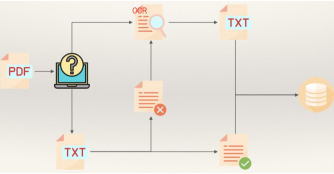
\includegraphics[width=13cm, center]{figuras/gpan-pipeline.png}
  \caption{Fluxo de processamento de processos do STF pelo GPAM.}
  \label{fig:gpan-pipeline}
\end{figure}

Nesse processamento, uma das etapas consistiu em verificar se a página do documento possui texto selecionável ou não, para então realizar a extração do texto via algoritmo de OCR. Tudo isso foi armazenado em um arquivo CSV, cuja as principais estão descritas a seguir.

\begin{table}[h]
 \centering
 \caption{Principais características do dado CSV}
 \begin{tabular}{|m{8em}|m{20em}|}
    \hline
    Coluna    &     Descrição \\
    \hline
    processo  &     teste \\
    \hline
    documento  &     teste \\
    \hline
    page\_is\_ocr  &     teste \\
    \hline
 \end{tabular}
 \label{tab:csv-details}
\end{table}

\subsection{Tratamento e formação do \textit{dataset}}

Por se tratar de uma problemática diferente do GPAM, foi preciso consumir o que foi fornecido e gerar novos dados que se encaixem melhor para a solução. Para tal, criou-se um conjunto de algoritmos para pegar os dados e realizar essa adequação no formato de uma \textit{pipeline}\footnote{
  Na computação, o termo \textit{pipeline} define um conjunto de processamentos de dados conectados em série, onde a saída de um desses elementos de processamento é a entrada do próximo, sendo elas dependentes para o processamento ser executado adequadamente.
}, com etapas de separação de documentos que possuem páginas que necessitam de OCR, extração de imagem a partir de PDF, criação de filtros de imagem e extração de informação de imagem utilizando o OCR.

\hl{DESENHAR FLUXO DE TRATAMENTO DE DADO}

\begin{itemize}
  \item \textbf{Separação de documentos:} o conjunto de PDFs fornecidos como dados estavam todos juntos em um único diretório no disco, sem a correta divisão de qual era o dado contido no PDF. O CSV fornecido pelo GPAN e os itens descritos na tabela \ref{tab:csv-details} fazem referência a todas as páginas desses PDFs e possui também o seu conteúdo, sendo eles extraídos por meio de OCR ou não, como mostra a figura \ref{fig:gpan-pipeline}. Porém como o foco do trabalho é realizar estudos sobre a qualidade do OCR, decidiu-se por separar o dado entre os que foram extraídos utilizando OCR dos que não foram.

  Para isso, gerou-se um novo CSV apenas com os registros de páginas cujo necessitou-se do OCR em sua extração e criou-se também um diretório para armazenar apenas os PDFs que possuíam páginas não-selecionáveis.
  \item \textbf{Extração de imagem:} com os dados separados em um diretório específico, iniciou-se a etapa de extração de imagem a partir dos documentos em formato PDF dos processos. Utilizou-se também informações do CSV (tabela \ref{tab:csv-details}) para selecionar a página específica do documento a qual o OCR foi utilizado, diminuindo assim o tempo de processamento por documento.

  A extração de imagem a partir do PDF é feita utilizando um algoritmo de software livre desenvolvido em Python, chamado de \textit{pdf2image}. Ele recebe como entrada um PDF e é possível definir qual ou quais páginas do PDF deseja-se extrair, permitindo assim a geração do \textit{dataset} de imagens de processos.
  \item Aplicação de filtros
  \item Extração de informação via OCR
\end{itemize}

\subsection{Criação de filtros}

\section{Método proposto}